% Created 2023-03-23 Thu 02:32
% Intended LaTeX compiler: pdflatex
\documentclass[a4paper,twocolumn]{article}
\usepackage[utf8]{inputenc}
\usepackage[T1]{fontenc}
\usepackage{graphicx}
\usepackage{longtable}
\usepackage{wrapfig}
\usepackage{rotating}
\usepackage[normalem]{ulem}
\usepackage{amsmath}
\usepackage{amssymb}
\usepackage{capt-of}
\usepackage{hyperref}
\usepackage{breakcites}
\usepackage{paralist}
\usepackage{amsmath}
\usepackage{biblatex}
\addbibresource{/home/dp/Documents/Research_paper_SFR/bibl/bibliography/bibliography.bib}
\usepackage{hyperref}
\usepackage{graphicx}
\usepackage{caption}
\usepackage{booktabs}
\usepackage[T1]{fontenc}
\usepackage{tgbonum}
\let\itemize\compactitem
\let\description\compactdesc
\let\enumerate\compactenum
\author{Dimitrios Papachistopoulos}
\date{\today}
\title{Investigations of the galaxies of the LCV}
\hypersetup{
 pdfauthor={Dimitrios Papachistopoulos},
 pdftitle={Investigations of the galaxies of the LCV},
 pdfkeywords={},
 pdfsubject={},
 pdfcreator={Emacs 28.2 (Org mode 9.6.1)}, 
 pdflang={English}}
\begin{document}

\maketitle

\section{The Galaxies in the Local Cosmological Volume (LCV)}
\label{sec:org50829b4}

The Catalogue of Neigbouring Galaxies (Karachentsev, Igor D. and Makarov  et al. 2013\autocite{karachentsevUPDATEDNEARBYGALAXY2013}) and its updated version from the ``Catalog \& Atlas of the LV galaxies'' databas\autocite{CatalogLVGalaxies}  are used to extract the K-band luminosities, the types of the galaxie\footnote{TType=Morphology type code according to the classification by de Vaucouleurs/ Tdw1=Dwarf galaxy morphology/ Tdw2=Dwarf galaxy surface brightness morphology}s, the mass within the Holmberg radius (M26), the Hydrogen masses of the galaxies (\(M_{HI}\)) and the SFRs based on integrated  H and far-ultraviolet (FUV) measurments for galaxies within a distance of
\(\approx 11\) Mpc. The SFR and MHI values contain limit flags, which we exclude from our present analysis. This gives a sample of 793 galaxies from 1248. From the remaing galaxies we have

\begin{table}[hc]
\centering
\begin{tabular}{lr}
\toprule
{} &    0 \\
\midrule
Name    &  793 \\
Kmag    &  321 \\
FUVmag  &  687 \\
TType   &  793 \\
Tdw1    &  580 \\
Tdw2    &  568 \\
Bmag    &  790 \\
SFR\_Ha  &  566 \\
SFR\_FUV &  688 \\
K       &  789 \\
MHI     &  643 \\
color   &  321 \\
\bottomrule
\end{tabular}
\end{table}

\begin{center}
\begin{tabular}{|l|l|}
\hline
Measurment & Number of Galaxies \\
\hline
\end{tabular}
\end{center}


The K-band values are converted to the total Stellar Masses of each galaxy according to the mass-to-light ratio of 0.6 (\cite{lelliSPARCMASSMODELS2016}), and the \(M_{HI}\) can be converted to the total mass of the gas of the galaxy using the equation \(M_g=1.33\,M_{HI}\)

The total SFR of each galaxy can be calcuated by

$$
    SFR_o=\frac{SFR_{FUV}+SFR_{Ha}}{2}
$$

if both \(SFR_{H\alpha},SFR_{FUV}\) measurments are available. If only one only one of them is given, then the SFR is equal to the given SFR value

$$
    SFR_o=SFR_i,\ \text{if } SFR_j=0,i\neq j,\ i,j=FUV, H_a
$$

The condition \(SFR_o\geq 10^{-3}M_\odot yr^{-1}\) leaves 579
galaxies. This condition is applied due to the reasons given in the P. Kroupa,M. Haslbauer, I. Banik, S. T. Nagesh and J. Pflamm-Altenburg et al. 2020 \cite{kroupaConstraintsStarFormation2020}

\section{Types of galaxies}
\label{sec:org54aef07}

Using the dataset of 1248 galaxies, do before using the condition and removing the galaxies with the flags, the below histograms can be plotted.

Most of the galaxies in the LCV are Higly Irregular galaxies followed by lenticular galaxies

Out of the 1248 galaxies the 1022 are dwarf galaxies


Most dwarf galaxies have low brightness and are irregulars followed by Dwarf spheroidal.

\begin{figure}[htbp]
\centering
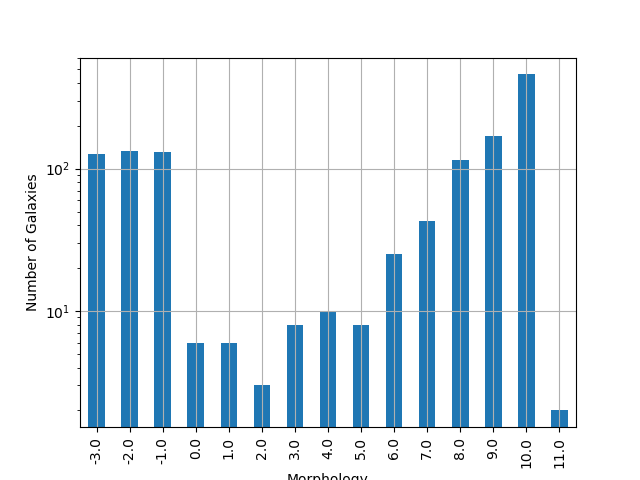
\includegraphics[width=.9\linewidth]{./figs/hist-Type.png}
\caption{\label{Types of galaxies}The classification by de Vaucouleurs et al. (1991) is used for the morphology of the galaxies}
\end{figure}

\begin{figure}[htbp]
\centering
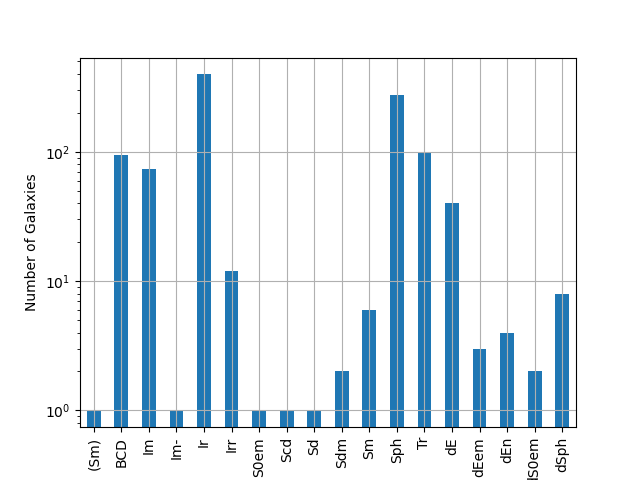
\includegraphics[width=.9\linewidth]{./figs/hist-Tdw1.png}
\caption{\label{Types of dwarf galaxies}Dwarf galaxy morphology}
\end{figure}

\begin{figure}[htbp]
\centering
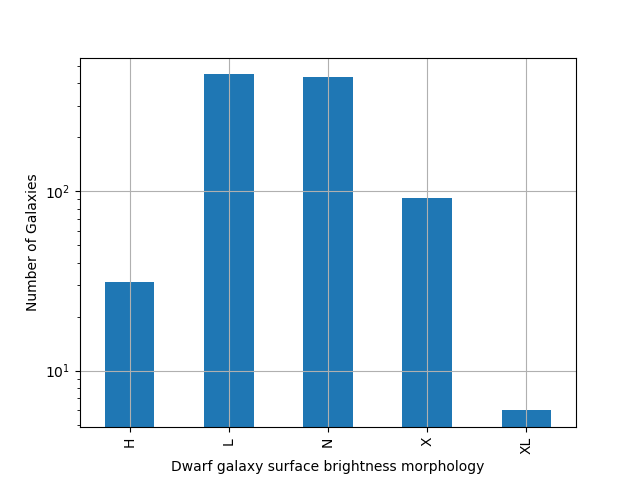
\includegraphics[width=.9\linewidth]{./figs/hist-Tdw2.png}
\caption{\label{Types of dwarf galaxies brightness}Dwarf galaxy surface brightness morphology, where: H = high; N = normal; L = low; X = extremely low.}
\end{figure}


\section{Delayed-\(\tau\) model}
\label{sec:org9d3ca76}

According to P. Kroupa et al. 2020\autocite{kroupaConstraintsStarFormation2020} current star formation rates of galaxies can be described by the 'delayed-\(\tau\)' mode as


\begin{equation} \label{eq:SFR}
SFR_{0,del}=\frac{A_{del}xe^{-x}}{\tau},\text{ where } x=\frac{t_{sf}}{\tau}
\end{equation}


where \(\tau\) is the star formation time-scale,  \(t_{sf}\) is the real time of star formation in a given galaxy and \(A_{del}\) a normalization constant.

The average SFR is

\begin{equation}\label{eq:av_SFR-x}
\overline{SFR_{del}}=\frac{A_{del}}{t_{sf}}[1-(1+x)e^{-x}]
\end{equation}
and can also be defined by the present day stellar mass

\begin{equation}\label{eq:av_SFR M*}
    \overline{SFR}=\frac{\zeta M_*}{t_{sf}}
\end{equation}
where \(\zeta\) accommodates for mass-loss through stella evolution and \(\zeta\approx 1.3\)

This is a system of 2 equations and 3 variables, since A\textsubscript{del} has never been calculated

\subsection{Constant \(t_{sf}\)}
\label{sec:orgb5e0687}
The observed ages of galactic discs are \(t_{sf}\approx 12\) Gyr\autocite{knoxSurveyCoolWhite1999}, so assuming an approximation of \(t_{sf}=12.5\) Gyr, the \(\overline{SFR_{del}}\) can be calcuated, from the equation (\ref{eq:av_SFR M*}).

After that the equation of ratio



\begin{equation} \label{eq:ratio}
    \frac{\overline{SFR_{del}}}{SFR_{0,del}}=\frac{e^x-x-1}{x^2}
\end{equation}

can be solved numerically for \(x\) and using the equations (\Ref{eq:SFR}) and (\Ref{eq:av_SFR-x}) the \(A_{del}\) and \(\tau\) of each galaxy are found.

\begin{table}[hc]
\centering
\begin{tabular}{lrrr}
\toprule
{} &    A\_tsf &      tau &    x\_tsf \\
\midrule
count & 5.78E+02 & 5.79E+02 & 5.79E+02 \\
mean  & 2.25E+12 & 1.09E+11 & 1.85E+00 \\
std   & 3.94E+13 & 1.04E+12 & 1.48E+00 \\
min   & 2.48E+07 & 1.93E+09 & 5.59E-04 \\
25\%   & 1.41E+08 & 4.18E+09 & 5.65E-01 \\
50\%   & 6.84E+08 & 7.79E+09 & 1.60E+00 \\
75\%   & 5.70E+09 & 2.21E+10 & 2.99E+00 \\
max   & 9.10E+14 & 2.24E+13 & 6.47E+00 \\
\bottomrule
\end{tabular}
\end{table}

\begin{figure}[htbp]
\centering
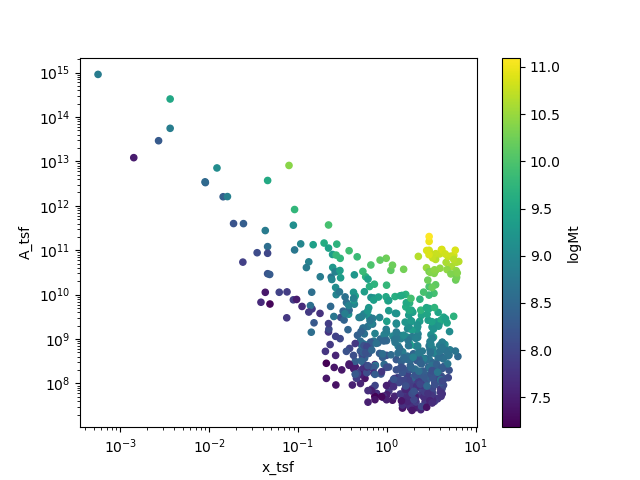
\includegraphics[width=.9\linewidth]{./figs/x-A_tsf.png}
\caption{\label{fig:$A_{del} = f(x)$ for constant t_{sf}}\(A_{del} = f(x)\) for constant t\textsubscript{sf}}
\end{figure}

\begin{center}
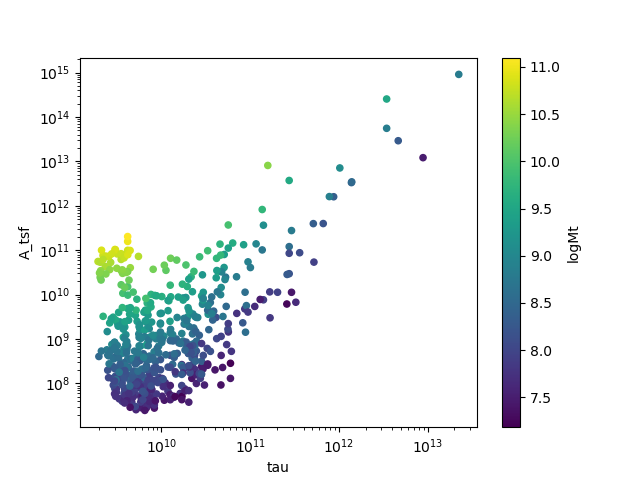
\includegraphics[width=.9\linewidth]{figs/T-A_tsf.png}
\end{center}


\subsection{Constant \(\tau\)}
\label{sec:org4942cfd}

Assuming for an constant \(\tau=3.5\) Gyr, we cannot use the same \(\overline{SFR}\) since it depends on \(t_{sf}\). Using the equations\textasciitilde{}(\Ref{eq:av_SFR M*}) and (\Ref{eq:ratio})

$$
    \frac{\overline{SFR_{del}}}{SFR_{0,del}}=\frac{e^x-x-1}{x^2}\Leftrightarrow \frac{e^x-x-1}{x}=\frac{\zeta M_*}{SFR\cdot\tau}
$$

using this equation \(x\) and \(A_{del}\) can be calcuated numerically.

\begin{table}[hc]
\centering
\begin{tabular}{lrrr}
\toprule
{} &    A\_tau &    x\_tau &      tsf \\
\midrule
count & 5.79E+02 & 5.79E+02 & 5.79E+02 \\
mean  & 4.59E+09 & 2.54E+00 & 8.89E+09 \\
std   & 1.50E+10 & 9.57E-01 & 3.35E+09 \\
min   & 9.87E+06 & 4.07E-01 & 1.42E+09 \\
25\%   & 6.50E+07 & 1.87E+00 & 6.55E+09 \\
50\%   & 2.37E+08 & 2.44E+00 & 8.54E+09 \\
75\%   & 1.12E+09 & 3.08E+00 & 1.08E+10 \\
max   & 1.06E+11 & 5.77E+00 & 2.02E+10 \\
\bottomrule
\end{tabular}
\end{table}

\begin{figure}[htbp]
\centering
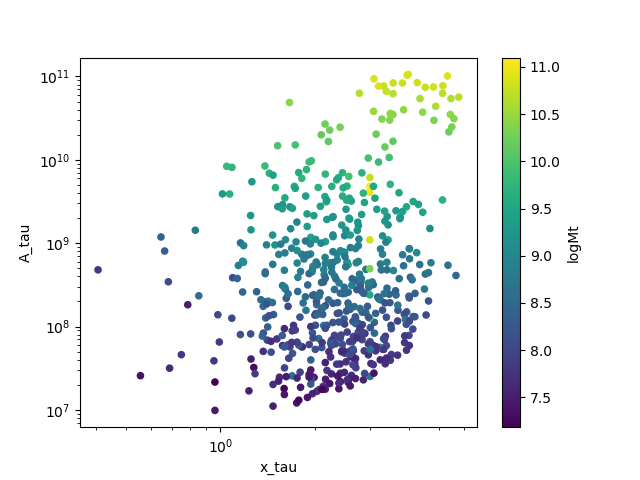
\includegraphics[width=.9\linewidth]{./figs/x-A_tau.png}
\caption{\label{fig:$A_{del} = f(x)$ for constant $\tau$}\(A_{del} = f(x)\) for constant \(\tau\)}
\end{figure}


\begin{center}
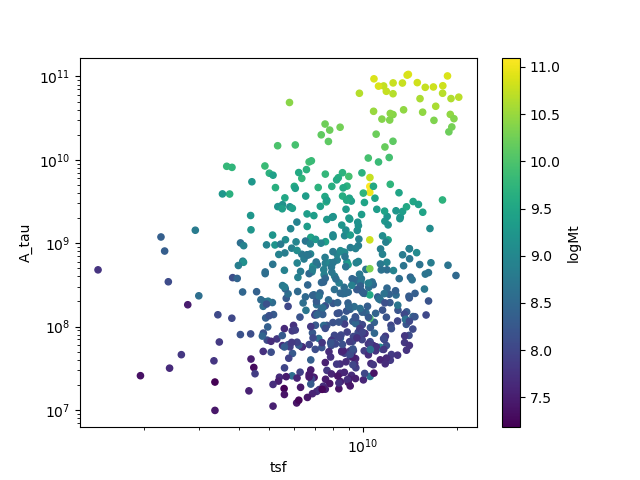
\includegraphics[width=.9\linewidth]{figs/T-A_tau.png}
\end{center}

\subsection{Comparing the two results}
\label{sec:org2d98e85}

\subsubsection{Comparing the \(x\)'s}
\label{sec:org7c16f4c}


Comparing the two different results for x, we see that the \(x|_\tau\) has a lower \(\sigma\)

\begin{table}[hc]
\centering
\begin{tabular}{lrr}
\toprule
{} &    x\_tau &    x\_tsf \\
\midrule
count & 5.79E+02 & 5.79E+02 \\
mean  & 2.54E+00 & 1.85E+00 \\
std   & 9.57E-01 & 1.48E+00 \\
min   & 4.07E-01 & 5.59E-04 \\
25\%   & 1.87E+00 & 5.65E-01 \\
50\%   & 2.44E+00 & 1.60E+00 \\
75\%   & 3.08E+00 & 2.99E+00 \\
max   & 5.77E+00 & 6.47E+00 \\
\bottomrule
\end{tabular}
\end{table}

\begin{figure}[htbp]
\centering
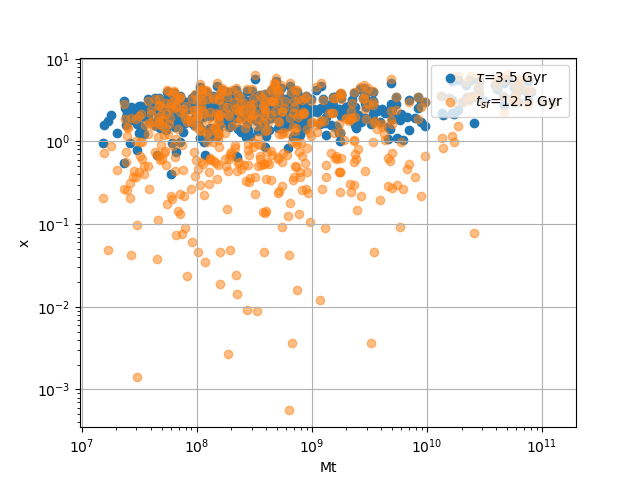
\includegraphics[width=.9\linewidth]{./figs/Comparing_the_x_Mt.png}
\caption{\label{fig:Comparing the two x's, According to their total masses}Comparing the two x's, According to their total masses}
\end{figure}
\begin{figure}[htbp]
\centering
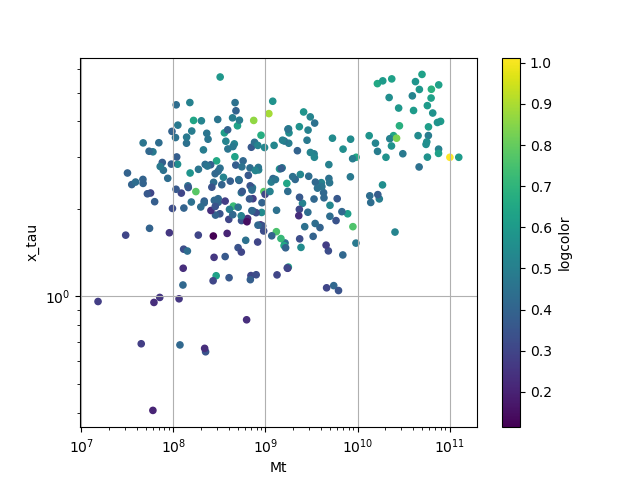
\includegraphics[width=.9\linewidth]{./figs/x_tau-Mt-color.png}
\caption{\label{fig:$x|_\tau=f(M_t)$, with their color index}\(x|_\tau=f(M_t)\), with their color index}
\end{figure}

\begin{figure}[htbp]
\centering
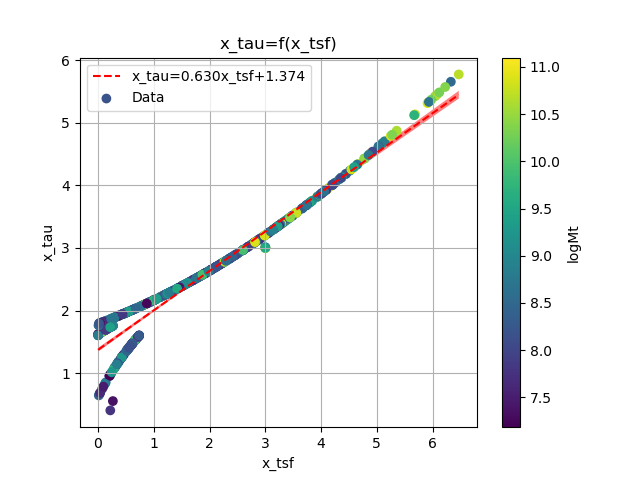
\includegraphics[width=.9\linewidth]{./figs/x_tsf-x_tau-color_logMt.png}
\caption{\label{fig:Comparing the two x, according to their total mass}Comparing the two x, according to their total mass}
\end{figure}

\begin{figure}[htbp]
\centering
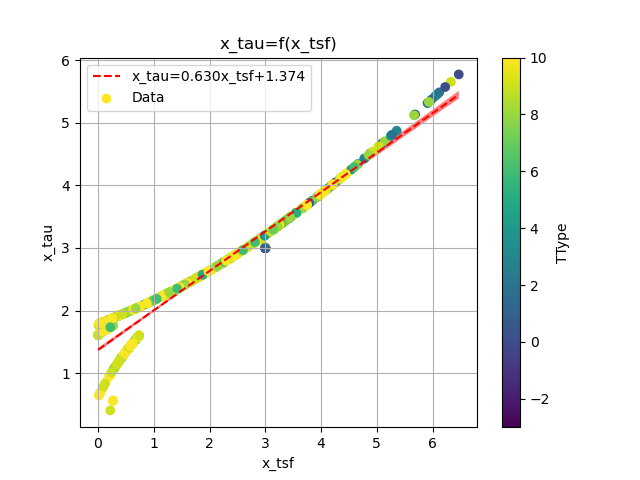
\includegraphics[width=.9\linewidth]{./figs/x_tsf-x_tau-color_TType.png}
\caption{\label{fig:Comparing the two x, according to their type}Comparing the two x, according to their type}
\end{figure}

\begin{figure}[htbp]
\centering
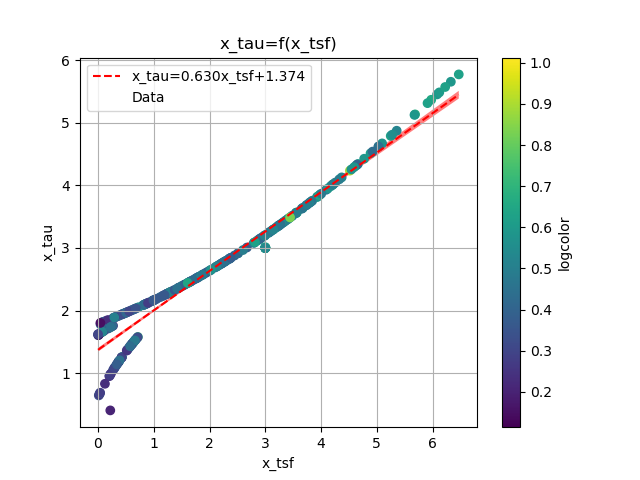
\includegraphics[width=.9\linewidth]{./figs/x_tsf-x_tau-color_logcolor.png}
\caption{\label{fig:Comparing the two x, according to their color index}Comparing the two x, according to their color index}
\end{figure}

The two results are interrelated through the equation:
\begin{equation}\label{eq:x_tsf-x_tau}
\begin{align}
& x|_\tau = (6.30(6) \times 10^{-1})\cdot x|_{tsf} + (1.374(15) \times 10^{0}) \\ 
& \textrm{with correlation } R^2=94\%
\end{align}
\end{equation}

and from the plots the following conclusions can be drawn:

\begin{enumerate}
\item The galaxies with a higher total mass deviate less from the linear fit and are older.
\item The younger galaxies are mainly later types of galaxies
\item For lower x's, the galaxies have a lower color index which indicates that they are younger. So the values are inline with the experimental values.
\end{enumerate}

\subsubsection{Comparing the normalization constants}
\label{sec:orgcf339e2}

\begin{figure}[htbp]
\centering
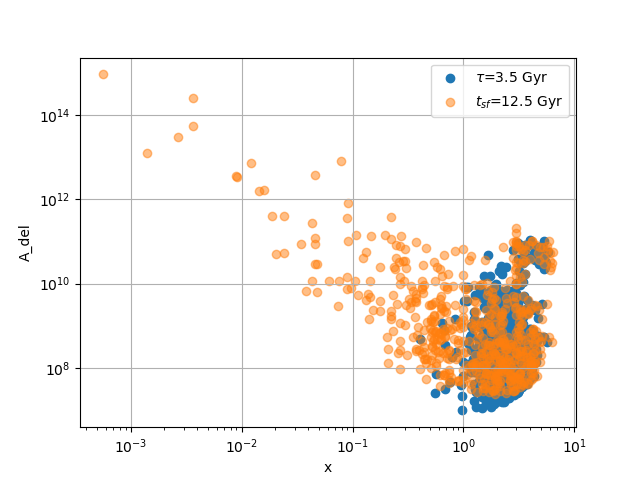
\includegraphics[width=.9\linewidth]{./figs/Comparing_the_A_x.png}
\caption{\label{fig:Comparing the two A_{del}}Comparing the two A\textsubscript{del}}
\end{figure}


\begin{figure}[htbp]
\centering
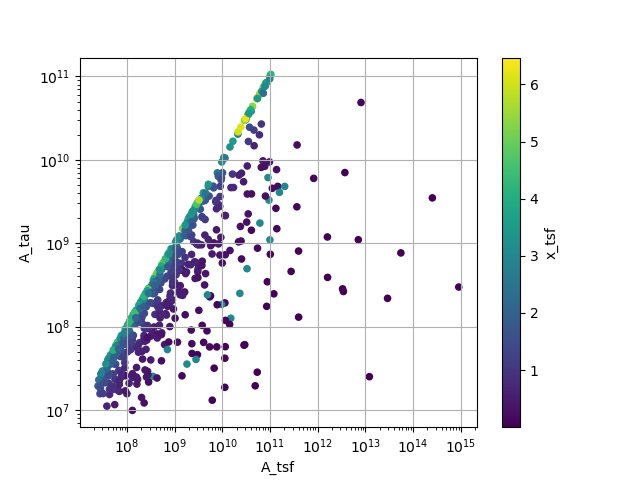
\includegraphics[width=.9\linewidth]{./figs/A_tau-A_tsf_colo_X.png}
\caption{\label{fig:Comparison of the 2 A_{del}s according to their $x$}Comparison of the 2 A\textsubscript{del}s according to their \(x\)}
\end{figure}
\begin{figure}[htbp]
\centering
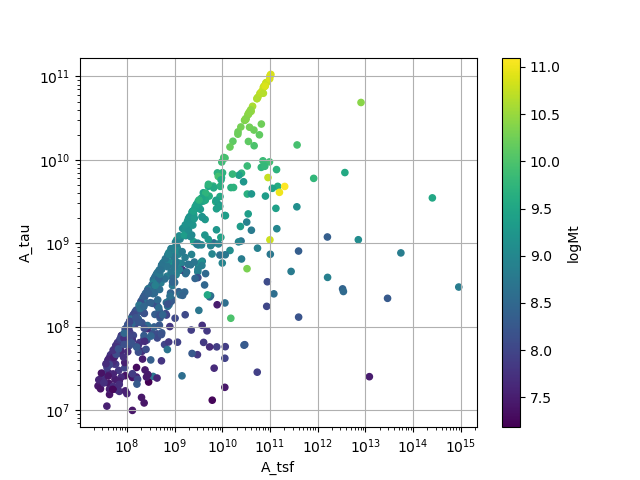
\includegraphics[width=.9\linewidth]{./figs/A_tau-A_tsf_Mt.png}
\caption{\label{fig:Comparison of the 2 A_{del}s according to their total masses}Comparison of the 2 A\textsubscript{del}s according to their total masses}
\end{figure}

For high \(x\) and high masses the two A\textsubscript{del}s have a high correlation. Specifically:
\begin{enumerate}
\item For high \(x\) the \(A_{del}|_{\tau}-A_{del}|_{t_{sf}}\) plot follows a \(y=x\) trend, which means that for older stars and stars with a low star formation timescale \(\tau\), the normalization constant is the same despite the method used to calculate it.
\item The same is true for more massive galaxies, since they deviate less from the \(y=x\) line
\end{enumerate}


\section{The gas depletion timescale \(\tau_g\)}
\label{sec:org33bc00a}

The gas depletion timescale \(\tau_g\) measures the time taken by a galaxy to exhaust its gas content Mg given the current SFR\autocites{nageshSimulationsStarformingMainsequence2023}[][]{pflamm-altenburgFundamentalGasDepletion2009}.
$$
\tau_g=\frac{M_g}{\dot{M_*}}=\frac{M_g}{SFR}
$$

\begin{figure}[htbp]
\centering
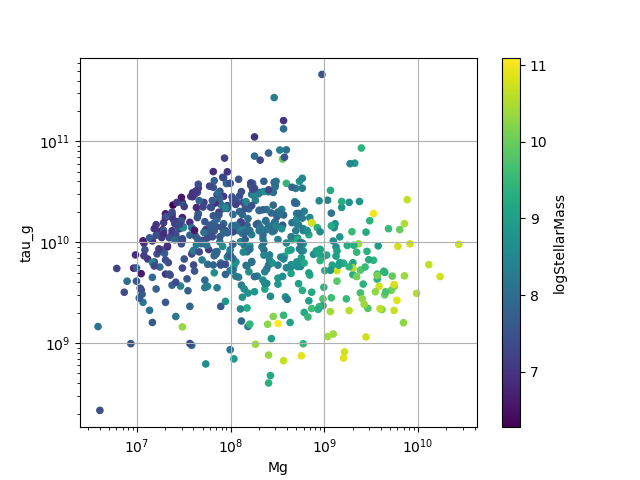
\includegraphics[width=.9\linewidth]{./figs/tau_g-Mg-color_StellarMass.png}
\caption{\label{fig:$\tau_g = f(M_g)$, with the Stellar Mass of the galaxies}\(\tau_g = f(M_g)\), with the Stellar Mass of the galaxies}
\end{figure}

\begin{figure}[htbp]
\centering
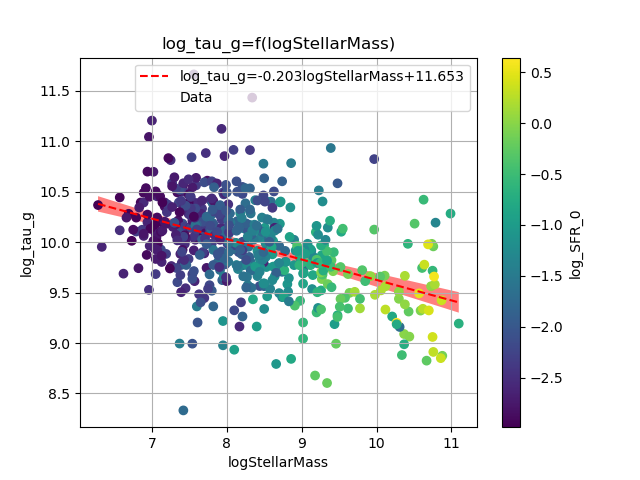
\includegraphics[width=.9\linewidth]{./figs/logStellarMass-log_tau_g-color_log_SFR_0.png}
\caption{\label{fig:Correlation of the $\tau_g$ with the SFR and the Stellar mass}Correlation of the \(\tau_g\) with the SFR and the Stellar mass}
\end{figure}

Even though the logarithmic correlation is low (\(R^2 = 21\%\)), there seems to be a pattern wherein the decrease of \(\tau_g\) corresponds to an increase in the values of the Stellar Mass and the current star formation \(SFR_0\).

\begin{figure}[htbp]
\centering
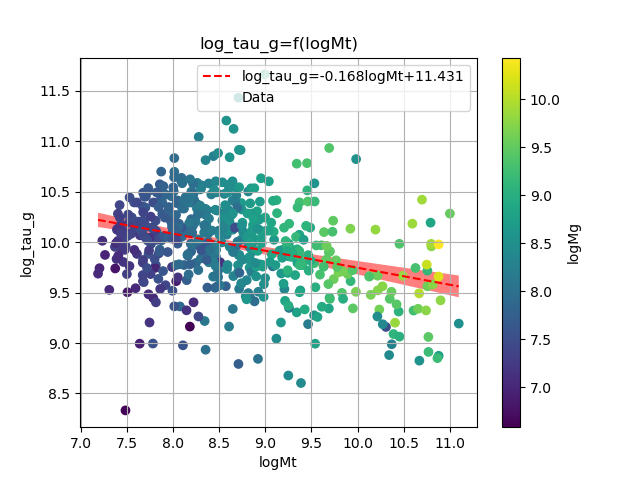
\includegraphics[width=.9\linewidth]{./figs/logMt-log_tau_g-color_logMg.png}
\caption{\label{fig:Correlation of the $\tau_g$ with the total mass and the mass of the gas}Correlation of the \(\tau_g\) with the total mass and the mass of the gas}
\end{figure}


Again it can be observed that as the \(\tau_g\) decreases, the corresponding values of \(M_t\) and \(M_g\) increase, but the logarithmic correlation is again low (\(R^2 = 11\%\)).

There is a notable trend, wherein for high masses we have a shorter timescale

\section{Mass relations}
\label{sec:org630e948}

Many of the galaxies masses have a high correlation with each other, and also help us undarstand the previous calculations.

\begin{figure}[htbp]
\centering
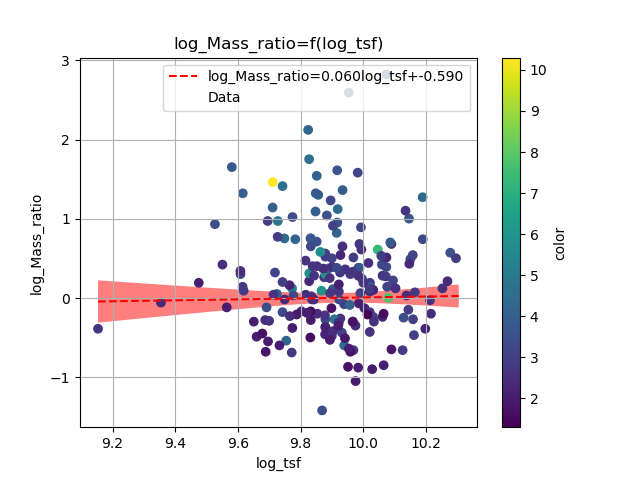
\includegraphics[width=.9\linewidth]{./figs/log_tsf-log_Mass_ratio-color_color.png}
\caption{\label{fig:None}None}
\end{figure}

As expected, the older the galaxy the mass ratio is higher, and the color index agrees ($\backslash$?)




\pagebreak
\printbibliography
\end{document}